Die Nacht haben wir Dank vierfach Schloss unverletzt überlebt und weil seit gestern das Auto meint wir sollten das Öl wechseln, haben wir den Ölstand kontrolliert.
Der hat gepasst und der Kundensupport meinte wir sollen uns nichts dabei denken und weiter fahren.
So haben wir das dann auch gemacht.\\

Gegen 10~Uhr waren wir wieder auf den Weg in den Yosemite National Park mit xxxxx Grove als Ziel.
Dort gab es Sequoia Bäume.
In etwa ein halbes Dutzend.
Die sind zum einen riesig, zum anderen feuerfest!
Sie brauchen die Waldbrände sogar, damit das Feuer die schneller wachsende Konkurrenz zu Dünger umwandelt und weil sich die Zapfen mit den Samen nur bei einem Brand öffnen.\\

Anschließend wollten wir über xxxxx und nicht wieder über Mariposa aus dem Park fahren, aber die Parkranger haben die andere Route vor unserer Nase dicht gemacht.
War sicherlich gesünder für uns, denn schneetauglich schien unsere Karre nicht zu sein.\\

Die Landschaft war in erster Linie wieder von Plantagen geprägt.
Kilometerweit ein Baum neben dem anderen, schön maschinengerecht in Reih und Glied angeordnet.
Im \glqq Zentrum\grqq \, lag die Ortschaft \TOWN{Orange Cove} und jetzt ist auch schon verraten, um was für Plantagen es sich handelte.
Am Plantageneingang fand sich noch die Warnung \FOREIGN{Spring Flood Area}, was bei dem erodierten Boden überhaupt kein Wunder ist.\\

Ein Arbeitskollege vom Christian hatte uns noch den \FOREIGN{Bass Lake} nahe \TOWN{Oakhurst} empfohlen.
Die Gegend war ja ganz nett, aber anscheinend waren wir auf der falschen, der zugebauten Uferseite.\\

Kurz vor \TOWN{Three Lakes} kamen wir noch an einem weiteren See vorbei, dem xxxxxx.
Das war bist jetzt die erste Anlage, die Besuchergebühren hatte.
War aber keiner da.

\thispagestyle{empty}
\begin{tikzpicture}[remember picture, overlay]
\node[inner sep=0pt, yshift=.25\paperheight] at (current page.south) {%
	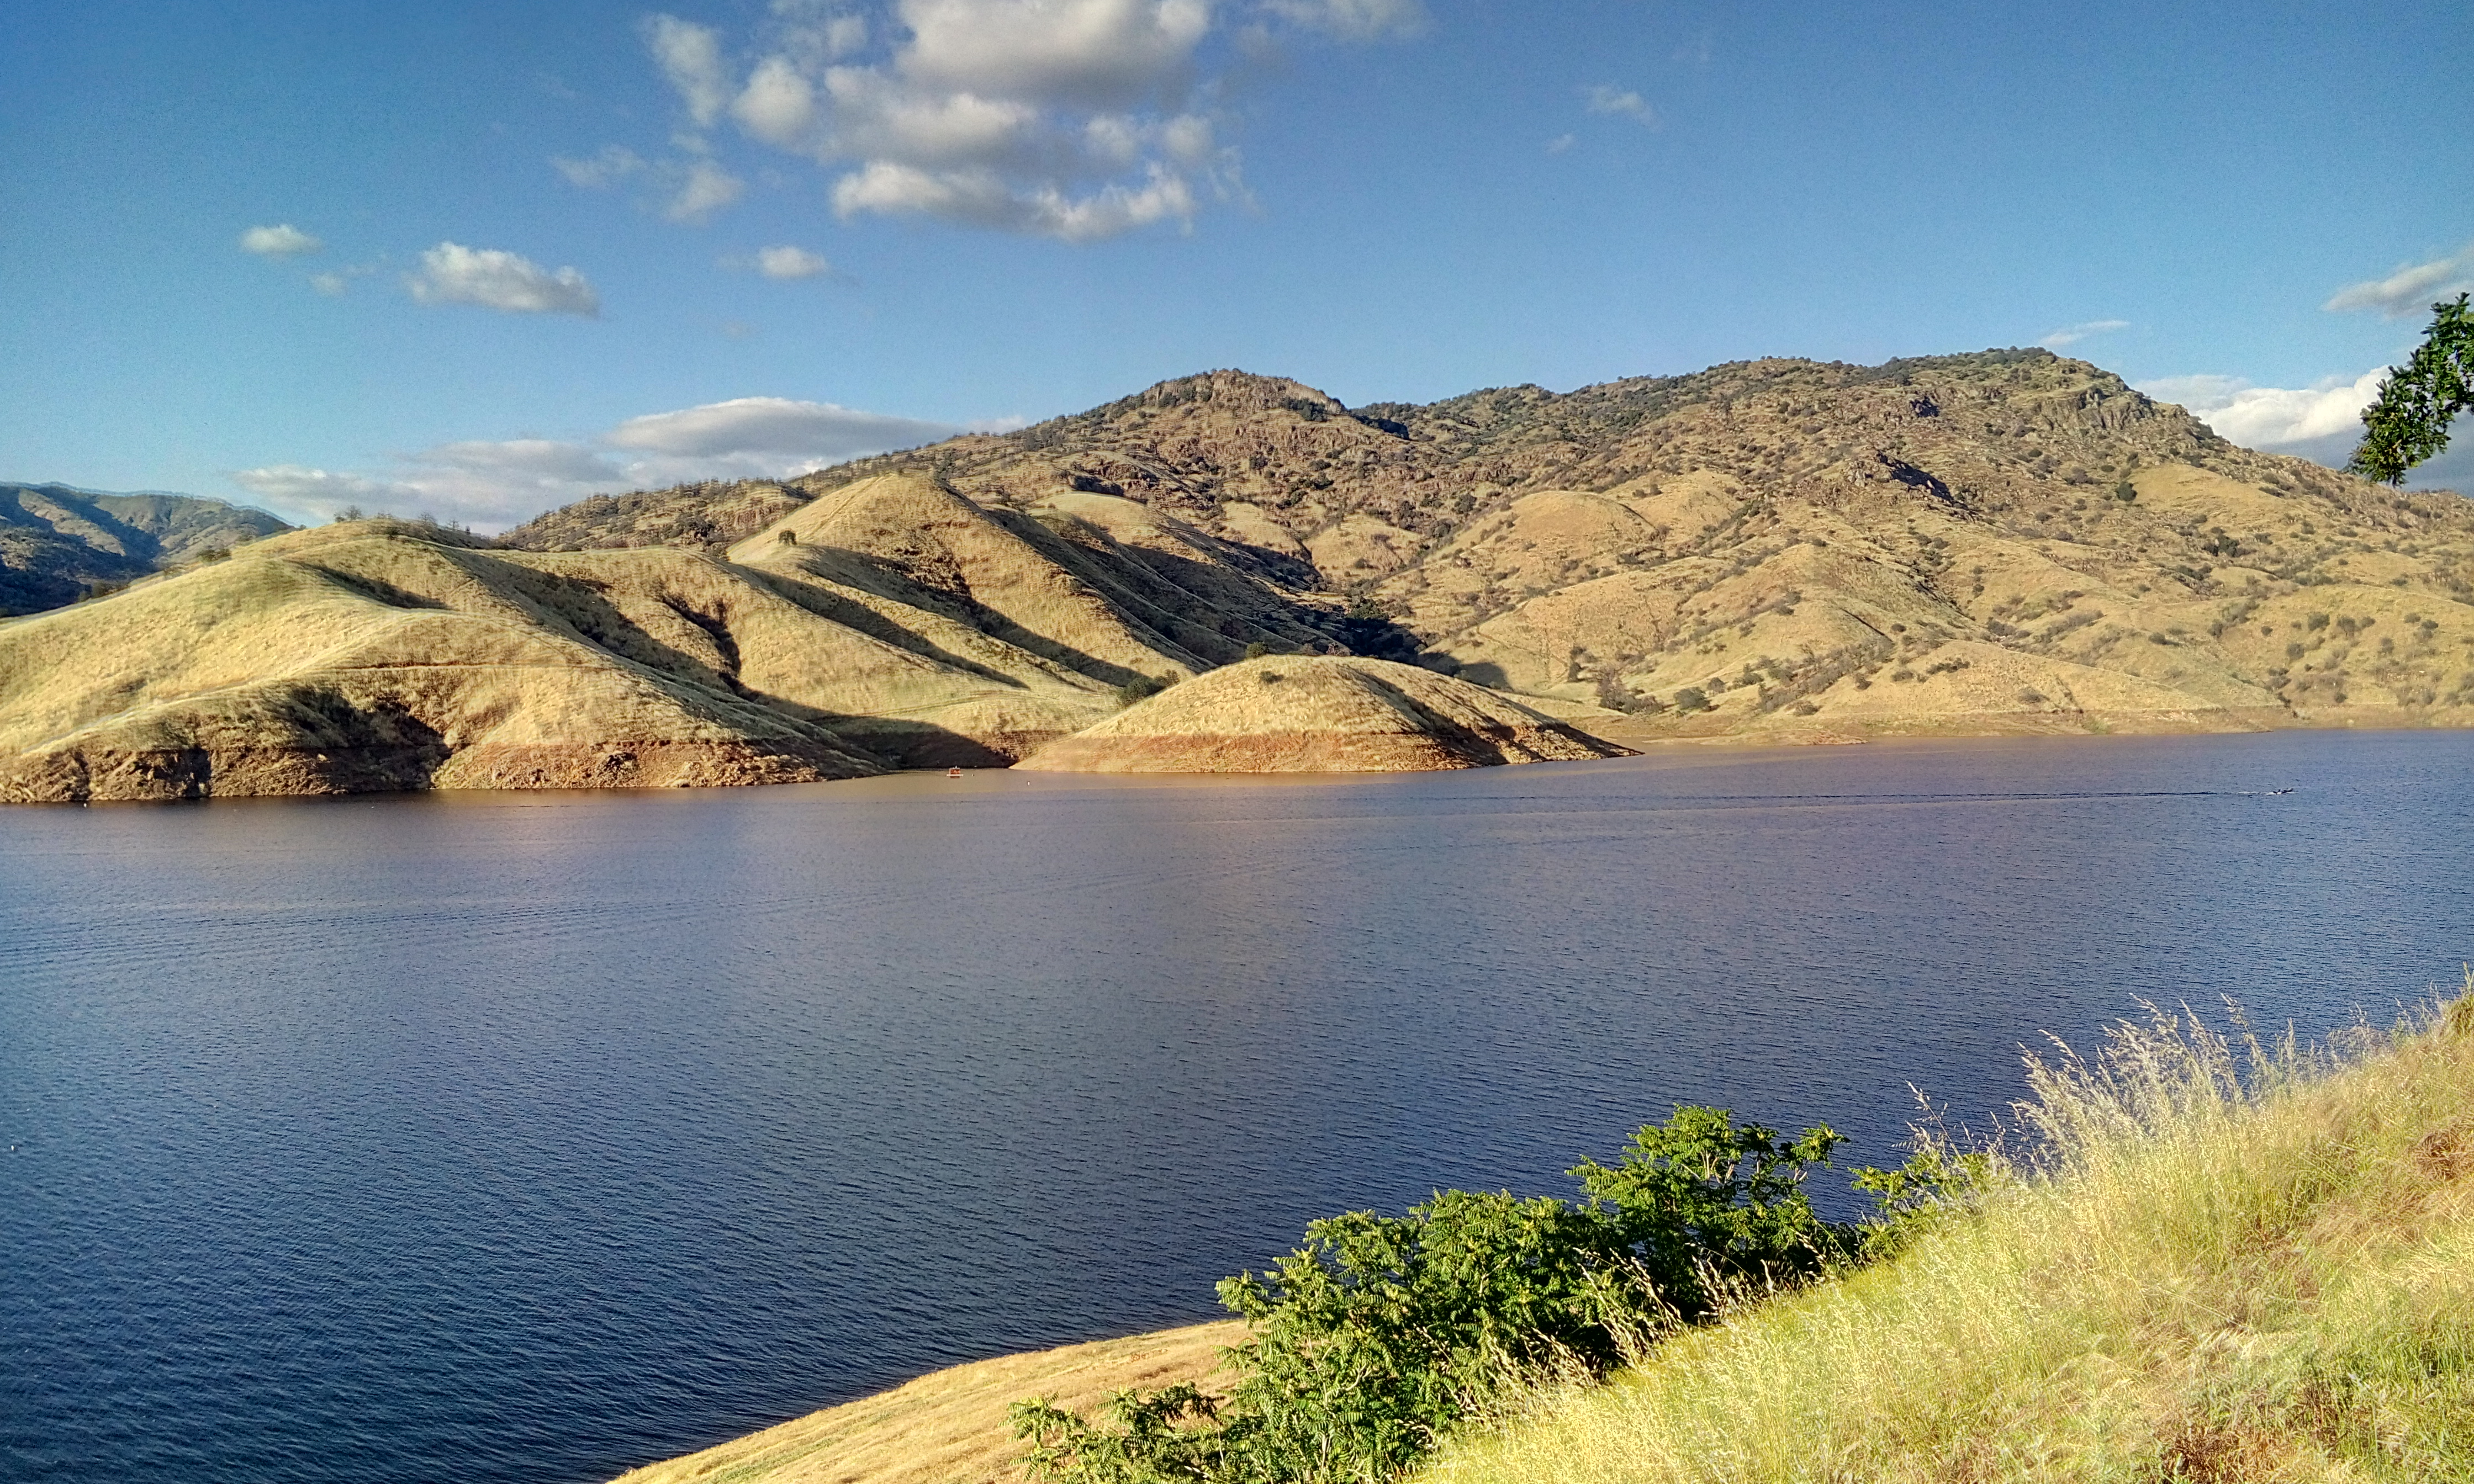
\includegraphics[angle=0,width=\paperwidth,height=.5\paperheight]{25/image20160425_182848870.jpg};%
};
\end{tikzpicture}
\newpage


In Oakhurst hatten wir gegen 14~Uhr unser Frühstück nachgeholt und da das auch noch bis in den späten Abend anhielt, substituierten wir das Abendessen durch Bier.
